\chapter{针对中医医案症状术语实体的识别}
\section{任务背景}
中华文明历史悠久,博大精深。
历经千年的传承与发展,古人为我们留下了许多文化艺术、科学技术的智慧结晶。
这些成果中有相当一部分以文字典籍的形式保留下来。
为了挖掘这些文字典籍中的知识和信息,在以文言文或文言、白话体文本混合的文本语料上进行处理尤其是命名实体识别任务,是中文自然语言处理中不可忽视的一部分。

在这些典籍中,我们选择了中医领域的典籍和医案,它们是中国传统医学宝贵的知识财富。
中医医案经历了长时间的积累,记载了古今众多医者的实证经验和临床诊疗规律。
这些医案中存在大量的症状信息,这些信息对医者辩证论治、察明证素,进而对证施治起着至关重要的作用;
同时,症状、治法、处方、剂量与预后疗效之间存在的内在联系,也能够反映中医对疾病的诊疗机理。
若要系统地研究这些诊疗机理,对医案进行结构化处理,挖掘医案文本,寻找其中蕴含的关联规则是一系列必要的任务。
在医案结构化处理任务中,首要的就是将中医医案文本中对症状具体的描述和长期以来形成的普遍使用的中医症状术语提取出来。

\subsection{中医医案症状术语识别的难点}
目前,针对中医医案文本中症状术语的识别存在几个难点。
首先,中医医案的结构化程度低。
具体表现为不同年代、不同地域的不同医家个体,其记录医案的结构和习惯均存在不同,导致无法按统一标准进行结构化。
其次,就医案内容而言,由于存在大量医案年代较为久远,其语言特点与现代汉语也存在较大差异,多为文言文或半文半白,识别难度较大。
最后,对于需要提取的目标症状描述或症状术语,缺乏统一的规范。
至今,中医临床常见症状术语尚未有国家标准,中医医案中口语化、症状实体包含、互指现象也十分普遍,加之症状描述本身形式灵活多变,这对识别症状的正确性、完整性提出了更高的要求。


\subsection{已有工作及其局限性}
识别中医医案文本中的症状描述或症状术语这一任务实际上就是从医案文本中进行症状实体识别,可以将其视为命名实体识别任务的一种。
目前对于中医医案症状识别主要使用CRF方法。
文献\citepns{王世昆2009基于条件随机场的中医命名实体识别}从命名实体识别的方法出发,对比了CRF与支持向量机、最大熵模型等常见的命名实体识别方法,指出了CRF在该任务上的有效性,但同时也存在依赖分词和词性标注效果、对超过五个字符的较长实体识别效果较差等局限性。
文献\citepns{刘凯2014基于条件随机场的中医临床病历命名实体抽取}对比了CRF、隐马尔科夫模型和最大熵隐马模型在特定病种的标准病历数据集上对症状、疾病和诱因的识别效果。
文献\citepns{孟洪宇2015基于条件随机场的《伤寒论》中医术语自动识别, 万静2016基于条件随机场的医药领域症状信息抽取, 叶辉2016基于多特征条件随机场的《金匮要略》症状药物信息抽取研究, 孟洪宇2014基于条件随机场的中医术语抽取方法及其应用探析}均采用了CRF方法针对中医领域的文本语料进行命名实体识别,以进行医案结构化、症状等中医术语提取等工作。

上述前人已有的工作,就识别方法而言存在一定局限性。
首先,选择传统的机器学习方法如最大熵、支持向量机和CRF等模型对较长症状的识别效果不佳\citep{王世昆2009基于条件随机场的中医命名实体识别}。
其次,这些方法对语料的结构化、标准化程度依赖较高,对大量非结构化的中医医案文本适应性较低,如文献\citepns{万静2016基于条件随机场的医药领域症状信息抽取}的训练语料来源是相对标准的、噪音较少的中医药物说明中的主治症状文本。
最后,使用CRF等模型同样依赖特征模板的构建,这对研究人员对领域数据的理解深刻程度提出了更高的要求,寻找、测试特征模板也将消耗较多的人力、时间成本。

本章针对上述局限性,提出使用结合神经网络的序列标注框架,
在以文言文本为主的近代中医医案典籍上进行中医症状术语识别,并根据症状组成要素,添加简单的字符级别特征,用字嵌入和症状字特征的联合向量代替原有一般的预训练字嵌入向量,在增加较少人工标注成本的前提下,获得更佳的症状识别效果。
本章将使用不同的LSTM结构进行实验,并对比分析不同结构对实验结果的影响,考察章节\ref{chap:3}介绍的标注模型在以文言文为主的语料上的效果。

\section{实验数据收集与预处理}
本章使用的数据集来自中医典籍《全国名医验案类方》,作者为近代名医何廉臣,共计492例医案。
原医案语料已具有一定的结构特征,但从逻辑上看,这些结构特征就是按照一定先后顺序出现的诊疗环节。
如单个医案中从诊疗缓解上划分了病因、证候、诊断、疗法、处方和预后效果等不同条目。
其中病因、诊断、证候和疗法属于在医者初次对病患进行四诊(望闻问切)时得到信息的记录以及对病情的分析。
这一部分中,诊断、证候和疗法包含较多症状术语。
而处方基本上只包括中药名称和剂量,不包含症状术语。
效果可以理解为预后,其中包含较多症状描述,因为在进行治疗后,患者的症状可能会减轻或病愈,也可能出现新的症状。
这些症状的描述都在效果中记载。
同时,医案中也存在大量多次诊疗的记录。
若某患者经过多次诊断、接受了多个处方药物的治疗,则这些内容将以“复诊”、“又方”、“三诊”、“三方”这样的形式依次出现在医案中,因此每一次诊断都包含对上一处方治疗效果的分析,包括哪些症状减轻或消失、哪些症状加重或出现等。

可以看出,中医医案中的文本信息量较大,具有很高的研究和挖掘价值。
但医案中也存在包括医者、病者等无关信息,因此本节只选取其中证候、诊断、疗法、效果及作为医案评述的“廉按”部分内容作为原始语料,共2959条语料。
原始语料文本示例如图\ref{fig:medical_case}

\begin{figure}[H]
    \centering
    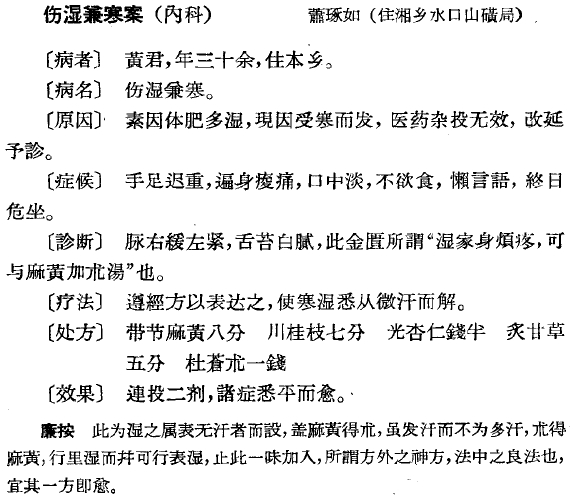
\includegraphics[width=0.8\textwidth]{Medical_case.png}
    \bicaption{医案原始文本}{Raw medical case text}
    \label{fig:medical_case}
\end{figure}
由于典籍中的医案是医者行医记录,虽然在医者已按照既定结构记载,但这些项目中仍存在大量描述和推断,不能完全作为症状实体。
且记录医案存在一定随意性,症状实体在证候、诊断、疗法、效果和医案评述中均可能出现,故对所有语料参考《中医临床症状术语规范》中六大类37小类共2069条规范症状进行标注。
考虑到原始语料年代较为久远,部分症状描述可能与现代汉语存在差异,故酌情对语料中频繁出现的部分症状进行了补充标注。

需要说明的是,文献\citepns{王世昆2009基于条件随机场的中医命名实体识别}和\citepns{万静2016基于条件随机场的医药领域症状信息抽取}的工作已经表明,对于中医医案尤其是使用古代汉语的中医医案语料,对其进行分词效果并不好,因为现有的分词工具多倾向于将无法识别的词语进行单字切分,若以词为粒度进行识别,分词会对结果产生负面影响。
因此本节利用字符级别特征进行序列标注,对所有语料进行单字切分,并按照BIO模式进行标注,即症状实体起始字标签为“B”,症状实体非起始字为“I”,非症状实体字为“O”。
由于实验语料规模较小,故实验中将随机抽取其中30例医案文本作为测试语料,剩余语料作为训练数据,其中训练集与验证集比例为9:1。

在预处理的过程中,我们主要进行了以下几个环节的处理:
\begin{enumerate}[leftmargin=*]
    \item[(1)] 数据清洗:整理数据文本编码和格式,标点符号以空格代替
    \item[(2)] 文本切分与预训练字嵌入:全文以字粒度进行切分,训练字嵌入向量,结果如图\ref{fig:TCM_charembeddings}所示
    \item[(3)] 数据标注:按照标注模式人工标注处理后语料中的症状术语
\end{enumerate}

\begin{figure}[H]
    \centering
    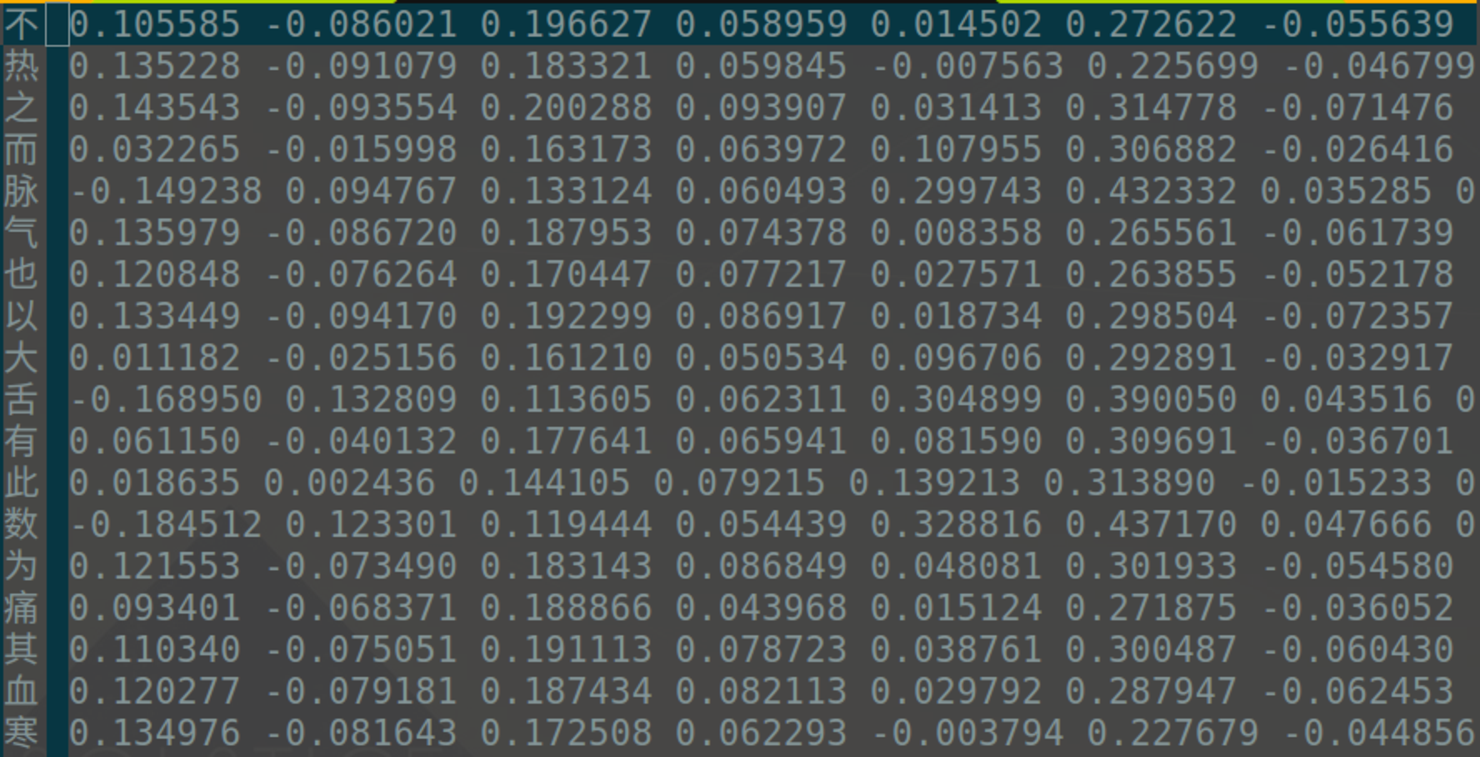
\includegraphics[width=0.8\textwidth]{TCM_charembeddings}
    \bicaption{由中医医案语料得到的字嵌入向量}{Character embeddings trained on TCM corpora }
    \label{fig:TCM_charembeddings}
\end{figure}

最后,为了得到相对较好的结果,实验中还使用Gensim工具利用全部中医医案语料作为训练数据,获得了预训练的字嵌入作为基本特征,字嵌入维度设置为100。
本章基于是否加入症状字特征和多种LSTM cell实现进行了对比实验。

\section{中医症状术语识别框架及改进}
一个基于双向LSTM-CRF框架的症状术语识别模型的训练算法以伪代码形式可以描述如算法\ref{alg:TCM_seq2seq_train}(以最基本的LSTM内部实现为例)所示。
\begin{algorithm}[H]
    \renewcommand{\algorithmicrequire}{\textbf{Input:}}
    \renewcommand{\algorithmicensure}{\textbf{Output:}}
    \caption{TCM Symptom Terminology Recognition Model Train Process}
    \label{alg:TCM_seq2seq_train}
    \begin{algorithmic}[1]
        \REQUIRE ~~\\
            Sentence sequences: $\Matrix{X}^{m}$\\
            Pre-trained embedding dict: $E$\\
            Entity label sequences: $\Tensor{Y}^{m}$
        \ENSURE ~~\\
            Model parameters stated in Chapter 3.
        \STATE Initiate $LSTM_{forward}$,$LSTM_{backward}$ and CRF layer parameter
        \FOR{Sentence $\Vector{x_i}\in \Matrix{X}^{m}, i\in [0, m]$}
            \STATE Initiate $\overleftarrow{h}_0$, $\overrightarrow{h}_0$
            \FOR{$t\in [1 \dots max\_sequence\_size]$}
                \STATE index $x_{it} \in \Vector{x_i}$
                \STATE current\_embedding $\Vector{x_{it}} \Leftarrow$ look up $x_{it}$ in $E$
                \STATE hidden layer output $\overrightarrow{\Vector{h}_{t}} \Leftarrow LSTM_{forward}(\Vector{x}_{it}, \Vector{h}_{t-1})$
                \STATE $\overrightarrow{\Matrix{h}} \Leftarrow \overrightarrow{\Matrix{h}}$ append $\overrightarrow{\Vector{h}_{t}}$
                \STATE Truncated BPTT or Full BPTT //Updates forward LSTM parameters.
            \ENDFOR
            \FOR{$t\in [max\_sequence\_size \dots 1]$}
                \STATE index $x_{it} \in \Vector{x_i}$
                \STATE current\_embedding $\Vector{x_{it}} \Leftarrow$ look up $x_{it}$ in $E$
                \STATE hidden layer output $\Matrix{h}_{t} \Leftarrow LSTM_{backward}(\Vector{x}_{it}, \Vector{h}_{t-1})$
                \STATE $\overleftarrow{\Matrix{h}} \Leftarrow \overleftarrow{\Matrix{h}}$ append $\overleftarrow{\Vector{h}_{t}}$
                \STATE Truncated BPTT or Full BPTT //Updates backward LSTM parameters.
            \ENDFOR
            \STATE $\Matrix{h} \Leftarrow element\_wise\_concat(\overrightarrow{\Matrix{h}},\overleftarrow{\Matrix{h}})$
            \STATE $\Matrix{P} \Leftarrow linear\_layer\_projection(\Matrix{h})$ 
            \STATE Maximize target function value as equation \ref{eq:log_likelyhood}
            \STATE Record loss on train set/validate set and update transition parameters in CRF
            \IF{loss on validate dataset reduces:}
                \STATE Save model parameters
            \ENDIF
        \ENDFOR
        \RETURN Model parameters
    \end{algorithmic}
\end{algorithm}

预测过程的算法描述与训练算法具有一定相似之处,只是初始化时读取模型参数,并在提供数据之后不再进行模型参数更新。
参照第三章介绍的预测过程给出最佳序列结果。具体算法如算法\ref{alg:TCM_seq2seq_predict}
\begin{algorithm}[H]
    \renewcommand{\algorithmicrequire}{\textbf{Input:}}
    \renewcommand{\algorithmicensure}{\textbf{Output:}}
    \caption{TCM Symptom Terminology Recognition Model Predict Process}
    \label{alg:TCM_seq2seq_predict}
    \begin{algorithmic}
        \REQUIRE ~~\\
            Sentence sequences: $\Matrix{X}^{m}$\\
            Pre-trained embedding dict: $E$\\
            Trained model parameters
        \ENSURE ~~\\
            Entity label index sequences: $\Matrix{V}$
        \STATE Load parameters from saved model
        \FOR{Sentence $\Vector{x_i}\in \Matrix{X}^{m}, i\in [0, m]$}
            \FOR{$t\in [1 \dots max\_sequence\_size]$}
                \STATE index $x_{it} \in \Vector{x_i}$
                \STATE current\_embedding $\Vector{x_{it}} \Leftarrow$ look up $x_{it}$ in $E$
                \STATE hidden layer output $\overrightarrow{\Vector{h}_{t}} \Leftarrow LSTM_{forward}(\Vector{x}_{it}, \Vector{h}_{t-1})$
                \STATE $\overrightarrow{\Matrix{h}} \Leftarrow \overrightarrow{\Matrix{h}}$ append $\overrightarrow{\Vector{h}_{t}}$
            \ENDFOR
            \FOR{$t\in [max\_sequence\_size \dots 1]$}
                \STATE index $x_{it} \in \Vector{x_i}$
                \STATE current\_embedding $\Vector{x_{it}} \Leftarrow$ look up $x_{it}$ in $E$
                \STATE hidden layer output $\Matrix{h}_{t} \Leftarrow LSTM_{backward}(\Vector{x}_{it}, \Vector{h}_{t-1})$
                \STATE $\overleftarrow{\Matrix{h}} \Leftarrow \overleftarrow{\Matrix{h}}$ append $\overleftarrow{\Vector{h}_{t}}$
            \ENDFOR
            \STATE $\Matrix{h} \Leftarrow element\_wise\_concat(\overrightarrow{\Matrix{h}},\overleftarrow{\Matrix{h}})$
            \STATE $\Matrix{P} \Leftarrow linear\_layer\_projection(\Matrix{h})$ 
            \STATE //Find $y*$ that maximizes $s(\Matrix{X},\Vector{y})$ as equation \ref{eq:sxy} using Viterbi algorithm
            \STATE $label\_sequence \Leftarrow viterbi(s(\Matrix{X},\Vector{y}), \Matrix{P})$
            \STATE $predict\_sequences \Leftarrow$ append $label\_sequence$
        \ENDFOR
        \RETURN $predict\_sequences$
    \end{algorithmic}
\end{algorithm}

考虑到中医症状实体本身还具有很多明显的特征,以这些特征作为锚点,能够快速准确地定位一些出现比较频繁的症状。
但同时也存在小部分负例,应以文本序列出现的上下文信息判断是否是症状。

\begin{table}[H]
    \centering
    \footnotesize
    \setlength{\tabcolsep}{4pt}
    \renewcommand{\arraystretch}{1.2}
    \bicaption{症状字特征分类}{Classes of symptom character features}
    \begin{tabular}{cp{5cm}c}
        \toprule
        特征种类 & 部分特征关键字 & 特征标签\\
        \midrule
        自感特征 & 疼、痛、肿、胀、酸、麻 & SF(self feeling)\\
        \midrule
        身体部位 & 脉、左、右、寸、关、尺、舌、苔、手、身、口、目、眼、耳、足、胸、额、头、脘、腹、唇、齿、胃、面、颊、肢 & BP(body parts)\\
        \midrule
        颜色形态 & 白、赤、红、滑、腻、溏、稀、干、燥、朱、黑、青、紫、绛、焦、黄 & CS(color shape)\\
        \midrule
        程度描述 & 稍、微、略、甚、强、大、多、少、无、极、弱 & AD(adverbs of degree) \\
        \midrule
        排泄物名词 & 便、溲、痰、汗 & EC(ecreta)\\
        \bottomrule
    \end{tabular}
    \label{tab:symptom_cluster}
\end{table}
为了考察这些特征对症状识别结果的影响,本节进行了如表\ref{tab:symptom_cluster}所示的特征标签分类。
对于文本序列中的单字,模型使用预训练的字嵌入作为基本特征;额外的症状术语单字,将采用随机初始化获得其表示其标签类型的嵌入向量,与字嵌入连接作为该字符的表示。
表\ref{tab:symptom_cluster}所示特征,仅为对标准化的症状词典进行简单的字符频率统计并按照字符表意类型进行分类得到的常见额外字特征。

上述特征均是字符级别。
为了不增加训练语料的人工标注成本,可以在训练语料中进行简单的单字替换获得,作为单独的特征列输入模型。
最终的标注结果示例如\ref{fig:character_level_feature}所示。

与单纯使用双向LSTM-CRF框架进行症状术语识别不同的是,本文将预训练的字嵌入$\Vector{char\_embedding}$和单字特征$\Vector{symptom\_feature}$进行连接获得的新的字向量表示作为模型输入,这些额外特征将作为字嵌入的扩展,为模型提取特征从而进行症状术语识别提供更具体有效的信息。
基于症状要素的字特征嵌入维度设置为30。
即在算法\ref{alg:TCM_seq2seq_train}中初始化参数时,增加单字特征随机初始化嵌入向量的过程,并在第7行使用$[\Vector{x_{it}},\Vector{symptom\_feature}]$代替原有的$\Vector{x_{it}}$。
\begin{figure}[H]
    \centering
    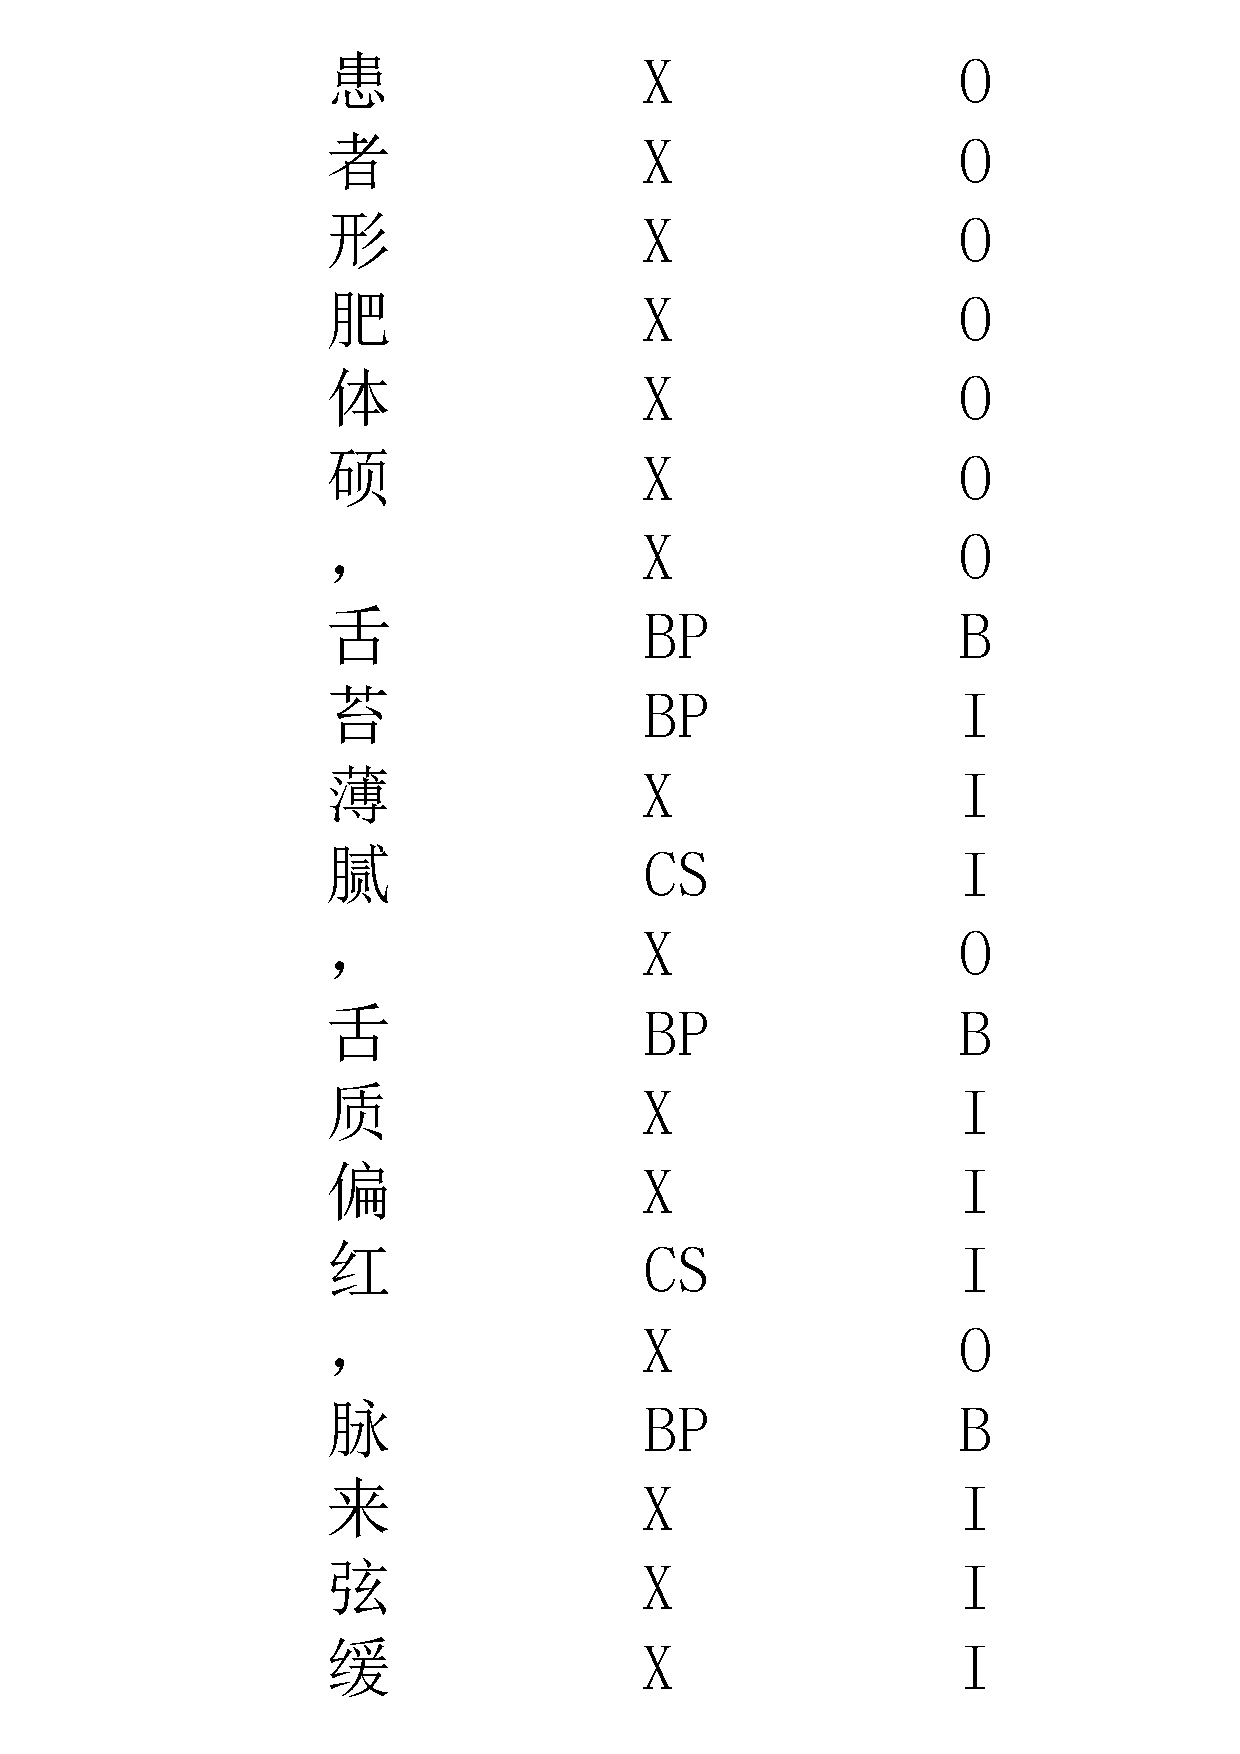
\includegraphics[width=0.5\textwidth]{Character-Level-Feature}
    \bicaption{增加字特征的医案标注文本示例}{Labeled examples of medical case with character features}
    \label{fig:character_level_feature}
\end{figure}


\section{整体架构}
根据章节\ref{chap:3}的介绍,我们基于双向LSTM-CRF框架构建了序列标注系统。

如图\ref{fig:TCM_NER}所示,输入特征为预训练词向量和字特征向量的连接。
LSTM层获取序列上下文特征,CRF层通过以上下文特征作为状态特征,同时训练标签转移矩阵参数,获得转移特征。
最后通过Viterbi算法在可行标签序列中,获得评分最高的序列作为最终预测序列输出。

整个序列标注系统逻辑上可分为四个模块:
\begin{enumerate}[leftmargin=*]
    \item[(1)] 数据预处理模块:进行数据清洗和预处理
    \item[(2)] 训练模块:训练得到模型参数
    \item[(3)] 预测模块:根据训练好的模型参数进行序列标注
    \item[(4)] 评估模块:评估模型效果,决策训练进程是否结束
\end{enumerate}
下面将具体介绍每个模块的主要功能,同时给出模型训练时的超参数设置。

\begin{figure}[H]
    \centering
    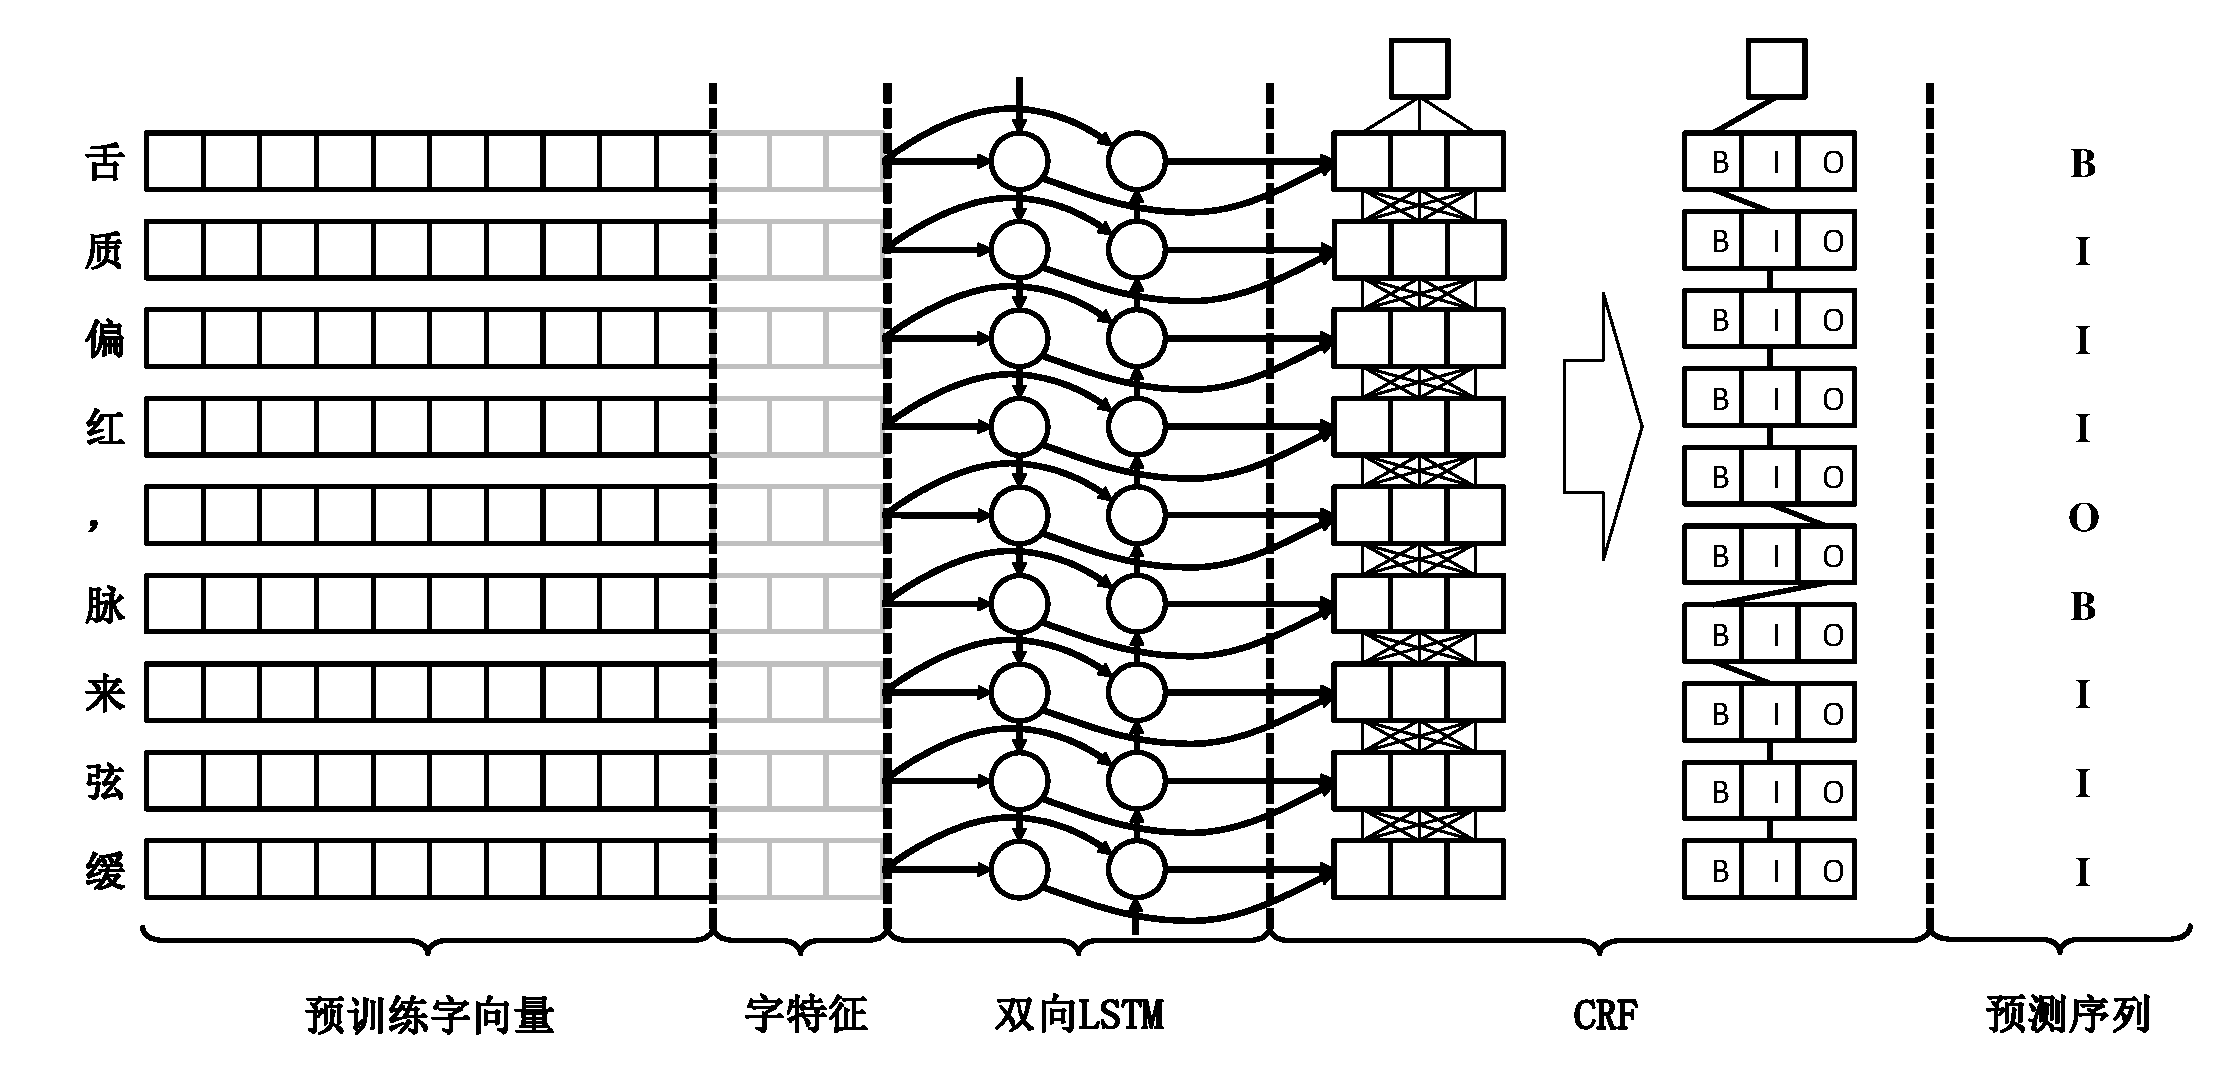
\includegraphics[width=\linewidth]{TCM-NER}
    \bicaption{双向LSTM-CRF中医医案症状术语标注框架结构}{Traditional Chinese medical case symptom labeling frame based on bi-LSTM-CRF}
    \label{fig:TCM_NER}
\end{figure}
\subsection{数据预处理模块}
首先,原始的语料数据需要进行下列处理才能成为模型训练可用的数据:
\begin{enumerate}[leftmargin=*]
    \item[(1)] 去除特殊字符:部分语料存在生僻字、弃用字和特殊符号等特殊字符,处理语料集时对影响语义的作替换处理,对不影响语义的作删除处理
    \item[(2)] 字符集统一:统一语料集文件字符编码,避免程序读取出错
    \item[(3)] 格式统一:统一标注结果格式,使其符合图\ref{fig:character_level_feature}所示的标注格式。
\end{enumerate}

同时还要以全部(未标注的)语料为训练语料,使用Gensim获取所有字的预训练字向量,获得字向量映射字典。
随后通过标注语料构建标签词典获取标签词典维度(标签类别数量),并记录字向量词典维度(字典大小)、字向量维度、句子长度(序列长度)和额外特征维度,这些参数将作为LSTM-CRF模型的初始化参数。
上述工作由数据预处理模块完成。
\subsection{训练模块}
模型内各权重参数的确定则是由训练模块负责。
训练模块包括两层实现:第一层是数据获取层,其作用是整合数据预处理模块提供的数据和模型初始化参数;第二层是模型层,根据第一层获得的模型初始化参数和预先设定的超参数,构建并初始化一个待训练的双向LSTM-CRF模型。
在模型构建的过程中,初始化了特征权重和特征的向量表示,并将字向量与其他特征向量表示形式顺序连接作为单字的嵌入。
在本章所述的场景下,额外的特征就是根据症状组成的元素标注的自感特征、身体部位、颜色形态等症状字特征。

对于LSTM层模型,本文对比了第三章所述的四种LSTM变体在中医症状术语识别上的效果。
此外在进行损失函数优化时选择了Adam优化器以适应高维字嵌入和可能存在的大数据量。

模型层中训练函数的实现即是在模型成功初始化后,将全部训练数据按一定比例随机分为测试集和验证集,并根据\verb|batch_size|的设置批量输入数据完成前后向传播的训练步,每一批数据对应的训练步结束之后更新模型权重矩阵,并同步计算该批次训练集上的训练损失函数均值和验证集上的损失函数均值。
验证集上的损失函数值将作为终止模型训练过程的重要依据。
在这一过程中,LSTM层的参数和CRF层中转移矩阵的参数在每一个\verb|batch|的训练后都将更新。
当损失函数值在验证集上经过一定批次的训练之后不再下降,或模型在一定批次的训练之后没有好于当前的最佳表现,则将停止训练。系统将保存表现在验证集上表现最佳的模型参数作为训练结果。

\subsection{预测模块}
预测模块主要负责根据训练好的模型参数来对待标注数据中的命名实体进行识别。
在待标记的测试数据集中,同样需要提供与训练集相同的特征数据,即字向量和特征向量(若存在额外特征)。

整个预测过程就是读取训练过程中保存的模型参数,使用训练好的参数和超参数实例化模型,随后将向量化的待标注数据输入模型,获得LSTM层输出的关于标签的概率向量,以及训练好的CRF层转移概率(即\ref{sssection:CRF}小节介绍的转移矩阵$\Matrix{A}$)。这时就可以根据式\ref{eq:CRF_predict},使用Viterbi算法求解概率最优序列。最后将这一序列转化为标签序列,得到了最终的命名实体识别结果。

\subsection{评估模块}
评估模块根据评价指标计算准确率、召回率和F值以评价模型在真实数据集上的识别效果。值得注意的是,由于本文讨论的方法均以字为基本单位,预测的结果也是字符级别的标签,一般而言对于公共领域语料的命名实体识别结果评估,其粒度是实体级别的,即完全匹配到实体才算正确识别。但对于中医症状术语的识别,以实体为粒度进行评估存在困难,因为就症状而言,存在较多的嵌套、并列等情况,因此我们参照已有工作,采用了与现有工作一致的评估标准,即以标签为粒度,这部份内容将在节\ref{sec:tcm-pfr}具体介绍。

评估模块的实现较为简单。对于以标签为粒度的评价指标,我们将标注结果与人工标注的结果进行比对即可得到准确率、召回率和F值。对于以实体为粒度的公共领域命名实体识别,我们首先分别对模型标注结果和人工标注结果进行处理,根据标签合并实体,最终统计实体数量并比对得到准确率、召回率和F值。

\subsection{超参数设置}
本节使用隐藏层单元的数量为64,训练语料句子长度最大不超过100个字符。
为防止过拟合,建立模型时对LSTM的输入层和输出层进行随机dropout,保留概率均设置为0.8。
同时,全连接层L2正则化参数为0.01,全局学习率为0.002。

\section{实验设计与评价指标}
\label{sec:tcm-pfr}
本章分别对基本LSTM单元、带peep-hole机制的LSTM单元、GRU和CIFG四种不同的LSTM实现进行了对比实验,并在此基础上增加了症状字特征进行实验。同时,本文将传统的CRF方法作为基线实验对比不同模型的效果。实验环境在Ubuntu 16.04LTS下使用CRF++v0.58,基本的特征模板示例如图\ref{fig:template}所示。CRF++所使用的训练数据格式与上文介绍的标注格式一致。
\begin{figure}[H]
    \centering
    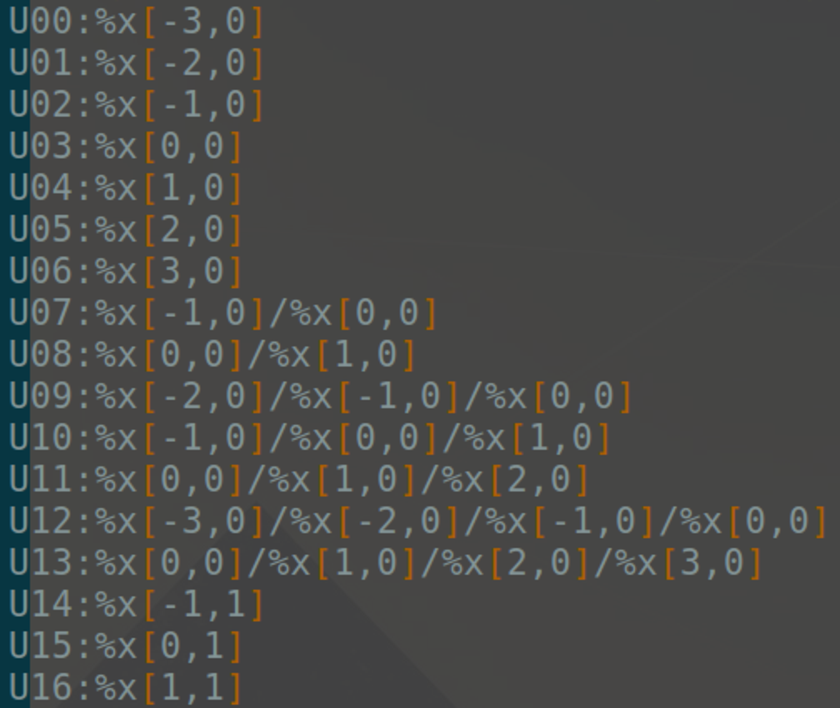
\includegraphics[width=0.5\textwidth]{templates}
    \bicaption{特征模板示例}{Example of feature templates}
    \label{fig:template}
\end{figure}
前面提到,中医症状术语既没有国家标准可以遵照,也没有公认的一套界定方案,因此其评价标准是按照一般命名实体整体对待,还是以字粒度为主,尚有待讨论。
且目前已有的在中医文本上进行命名实体识别的工作,多采用字符级别特征。

参考文献\citepns{万静2016基于条件随机场的医药领域症状信息抽取},我们选择以标签为对象的评价标准。实验结果以标签为粒度,对BI标签分别按表\ref{tab:confusion}统计准确率(Precision)、召回率(Recall)和F1值。
分别统计得到B、I的$TP$、$FP$、$FN$后,则两种标签的准确率$Precision$、召回率$Recall$和F值可以由式\ref{eq:preision}-\ref{eq:f-measure}计算。

\begin{equation}
    Precision = \frac{TP}{TP+FP} \label{eq:preision}
\end{equation}
\begin{equation}
    Recall = \frac{TP}{TP+FN}
\end{equation}
\begin{equation}
    F_\beta = \frac{(1 + \beta^2)\times Precision \times Recall}{(\beta^2\times Precision) + Recall}\label{eq:f-measure}
\end{equation}

\begin{table}[H]
    \centering
    \bicaption{混淆矩阵}{Confusion matrix}
    \begin{tabular}{ccc}
        \toprule
        \diagbox{真实结果}{预测结果} & 正类 & 负类\\
        \midrule
        正类 & True Positive (TP) & False Negative (FN)\\
        负类 & False Positive (FP) & True Negative (TN)\\
        \bottomrule
    \end{tabular}
    \label{tab:confusion}
\end{table}

其中$\beta$是正实数,表示$Precision$相对$Recall$的重要性。本节实验取$\beta = 1$。

\section{实验结果与分析}
本文以传统的CRF方法作为基线实验,分别在未加入和加入字特征的条件下进行对比实验。
实验结果如表\ref{tab:tab1}所示。其中,标$*$号行为未加入症状字特征的实验数据。
实验结果表明,基于LSTM-CRF的序列标注模型在中医医案症状识别任务中F1值最好达到了0.78。

在对中医医案进行序列标注的任务中,提高召回率是一个难点,这与文献\citepns{王世昆2009基于条件随机场的中医命名实体识别}相似语料上的实验得出的结论一致。
在未加入症状字特征的条件下,得益于相对简单的结构和较少的待训练参数,GRU取得了相对较好的识别效果。
增加症状字特征后,可以看出不同的LSTM实现在标签识别的效果上均有不同程度的提高,说明常见症状字特征对识别结果有一定的积极影响。

\begin{table}[H]
    \centering
    \bicaption{加入症状字特征识别效果对比}{Comparison on recognition results with or without character features}
    \begin{tabular}{cccccccccc}
        \toprule
            \multirow{2}{*}{Cell} &\multicolumn{3}{c}{Overall} &\multicolumn{3}{c}{B} &\multicolumn{3}{c}{I}\\
            \cmidrule(lr){2-4} \cmidrule(lr){5-7} \cmidrule(lr){8-10}
            & F1 & R & P & F1 & R & P & F1 & R & P\\
        \midrule
            CRF & *0.667 & 0.572 & 0.798 & 0.677 & 0.575 & 0.824 & 0.662 & 0.552 & 0.828\\
            CRF & 0.694 & 0.597 & 0.828 & 0.667 & 0.553 & 0.840 & 0.705 & 0.599 & 0.857\\
        \midrule
            LSTM & *0.724 & 0.621 & 0.866 & 0.736 & 0.635 & 0.874 & 0.718 & 0.600 & 0.894\\
            (basic) & 0.756 & 0.675 & 0.860 & 0.763 & 0.685 & 0.862 & 0.753 & 0.653 & 0.889\\
            LSTM & *0.748 & 0.691 & 0.815 & 0.746 & 0.689 & 0.812 & 0.748 & 0.670 & 0.848\\
            (peep-hole) & 0.763 & 0.699 & 0.839 & 0.748 & 0.685 & 0.824 & 0.769 & 0.687 & 0.873\\
            \multirow{2}{2cm}{\centering{GRU}} & *0.754 & 0.717 & 0.796 & 0.738 & 0.689 & 0.794 & 0.761 & 0.698 & 0.835\\
                                 & 0.762 & 0.708 & 0.825 & 0.758 & 0.707 & 0.816 & 0.764 & 0.687 & 0.861\\
            \multirow{2}{2cm}{\centering{CIFG}} & *0.742 & 0.664 & 0.839 & 0.749 & 0.662 & 0.863 & 0.738 & 0.640 & 0.872\\
                                  & 0.780 & 0.735 & 0.832 & 0.762 & 0.707 & 0.826 & 0.788 & 0.725 & 0.863\\
        \bottomrule
    \end{tabular}
    \label{tab:tab1}
\end{table}

其中,典型症状如脉象、舌象等具有较为明显的特征,其上下文也相对简单,故识别效果较好;经过比对发现,未识别正确的症状如内部存在递进等语义关系的“六脉俱缓,左关尤甚”、存在时间特征的“继则全体大热,昼夜不休”等,其症状形式较为多变,标准难以统一,这也造成了许多类似症状识别的困难。

另外,CIFG在加入症状字特征后,各标签的召回率和精确率都得到了提高。
也可以看出,与基本的LSTM单元实现相比,LSTM(with peep-hole)、GRU和CIFG三种带有peep-hole实现的单元结构对增加的特征更加敏感,特征对提升它们在症状实体识别任务上的表现具有更明显的作用。
与传统的CRF方法相比,LSTM-CRF框架省略了特征模板制定这一环节,而CRF的识别效果比较依赖人工的特征模板选择,在给定多列特征的情况下,特征模板也趋于复杂,优化模型效果较为耗时。

加入特征后,我们发现CRF模型的识别效果在部分指标上出现了下降。
本文认为出现这种结果主要是因为:
\begin{enumerate}[leftmargin=*]
    \item[(1)] 症状字特征与一般命名实体识别任务下加入的词性等额外特征等存在较大差异。
        词性标签在序列中前后存在较大依赖,其规律性较为明显;
        而症状字特征标记的是症状中的关键要素,这些要素在症状中出现的位置灵活多变,局部存在的依赖相对较弱,因此其特征较难展现。
    \item[(2)] 限于特征模板的选择,模型不能完全利用这些特征进行标注
\end{enumerate}

同时,使用LSTM-CRF序列标注模型相比单纯的CRF能够更好地识别较长的症状术语,改善了CRF对长症状术语不能很好召回的情况\citep{王世昆2009基于条件随机场的中医命名实体识别}。
各方法对测试语料中五字以上长症状术语的识别效果如表\ref{tab:tab2}所示。

\begin{table}[H]
    \centering
    \bicaption{LSTM-CRF对长症状术语的识别效果}{Long symptom recognition results using LSTM-CRF}
    \begin{tabular}{ccccccc}
        \toprule
            \multirow{2}{*}{Cell} & \multicolumn{3}{c}{B} & \multicolumn{3}{c}{I}\\
            \cmidrule(lr){2-4} \cmidrule(lr){5-7}
            & F1 & R & P & F1 & R & P\\
        \midrule
        {LSTM}{(baseline)} & 0.744&0.612&0.950&0.744&0.600&0.979\\
        {LSTM}{(peep-hole)} & 0.769&0.645&0.952&0.755&0.625&0.952\\
        {GRU} & 0.693&0.548&0.944&0.668&0.518&0.943\\
        {CIFG} & 0.754&0.645&0.909&0.770&0.643&0.962\\
        \bottomrule
    \end{tabular}
    \label{tab:tab2}
\end{table}

\section{本章小结}
本章在基于LSTM-CRF序列标注模型的基础上,针对中医症状特征添加了部分字符级别的要素特征,在小规模以古汉语为主的中医医案语料上的实验表明,该模型泛化能力更强,且对较长实体的识别效果更好。
同时,由于中医症状种类繁多,加之古汉语精干灵活的语言特点,该方法也存在召回率较低的缺点。
因此后续工作将围绕以下几点展开:第一,比较多种不同的标签模式对症状术语识别的效果影响;第二,由于部分症状描述分散于多个短语中,并且存在大量比较(如“六脉俱缓,左关尤甚”)、持续(如“继则全体大热,昼夜不休”)等特征,寻找有效方法利用这些特征也至关重要;最后还需考虑参照症状字典对不标准的症状描述进行聚类,识别时按照标准症状建立自然语言序列与症状的映射关系,便于以后对古医案的结构化。



